
\section{Recommender systems}

\paragraph{Definition.} Given a user and a set of items, a recommender system is a function that helps to match users with items by ranking the items in order of decreasing relevance.

We can discern two paradigms for recommender systems: 
\begin{itemize}
  \item \textbf{Collaborative:} tell me what other people like
  \item \textbf{Content-based:} show me more of what I liked from my past ratings and the data of these objects
\end{itemize}

\subsection{Collaborative user based filtering}

Widely used by large e-commerce sites, applicable in many domains. Users give ratings to items, we assume that users with similar tastes in the past will have similar tastes in the future.

\paragraph{Problems.} Cold start, scalability, more users than items (huge neighborhood), data dispersion (hard to find neighborhood). Possible solution: compute predictions offline and use learned model online + update model regularly.

\paragraph{Technique.} Given a user $U$ and an item $I$ not rated by $U$, estimate the rating $r_U(I)$

\begin{enumerate}
  \item Find a set of users $N_u$ who liked the same items as $U$ in the past and who have rated $I$
  \item Aggregate the ratings of $I$ provided by $N_U$ to get $r_U(I)$
  \item Compute the ratings for all the items not rated by $U$ and recommend the best-rated ones 
\end{enumerate}

\subsubsection{Similarity metric}
We need a metric to compute similarity between users and find the closest neighborhood of a user. 

\paragraph{Pearson correlation coefficient} as similarity measure. Given two users $x$ and $y$, a set of items $I$ rated by both $x$ and $y$ ($|I| = N$), and $r_x(i)$ the rating of $x$ for $i\in I$, the Pearson correlation coefficient is given by
\[
  \text{sim}_{corr}(x,y) = \frac {\sum_{i=1}^N (r_x(i)-\bar r_x)(r_y(i) - \bar r_y) } { \sqrt {\sum_{i=1}^N (r_x(i) - \bar r_x)^2} \sqrt {\sum_{i=1}^N (r_y(i) - \bar r_y)^2}}
\]
We have $-1 \leq \text{sim}(x,y) \leq 1$


\paragraph{Cosine similarity.} It consider each user as a $N$ length vector and compute the angle between $\mathbf{x}$ and $\mathbf{y}$. If angle is 0 the two ratings are very close (sim returns 1), if the vetors are orthogonal it return 0.

\[
  \text{sim}_{cos}(x,y) = \frac {\sum_{i=1}^N r_x(i)r_y(i)}{\sqrt{\sum_{i=1}^N r_x(i)^2} \sqrt{\sum_{i=1}^N r_y(i)^2}}
\]

One drawback of Pearson correlation coefficient is that it is not computable if the variance of one of the user ratings is 0 (e.g. a user with ratings 1 1 1 1). However, in general, the correlation coefficient works well in usual domains, compared to the cosine similarity. The reason is that the cosine similarity does not consider the magnitude of the ratings but only the angle between the vectors.

\subsubsection{Aggregate the ratings}

The following aggregation function is a weighted average using the similarity as a weight

\[
  r_x(a) = \bar r_x + \frac {\sum_{y \in N_x} \text{sim}(x,y)(r_y(a) - \bar r_y)} {\sum_{y \in N_x} |\text{sim}(x,y)|}
\]

\subsection{Item-based collaborative filtering}

We use the similarity between items (and not users) to make predictions. Given a user $U$ and an item $I$ not rated by $U$, estimate the rating $r_U(I)$:

\begin{enumerate}
  \item Find a set of items $N_I$ who are similar to $I$ and that have been rated by $U$
  \item Aggregate the ratings of the items in $N_I$ and use the aggregation as prediction of $r_U(I)$
\end{enumerate}

Be careful that in this technique the similarity between objects is computed only with regard to the rating given by users (two objects are similar if they have been graded the same way by the users). We don't use the content/description of the object (yet).

\paragraph{Aggregate the ratings.}

\[
  r_x(a) = \frac{\sum_{b\in N_a} \text{sim}(a,b) r_x(b)}{\sum_{b\in N_a} |\text{sim}(a,b)|}
\]

There is still the scalability problem but we can calculate all the pair-wise item similarities in advance. Items similarities are more stable and we only need to consider the neighborhood (small) at runtime.

\subsection{Content-based recommendation}

\begin{enumerate}
  \item Find the items that are similar to the past rated items
  \item Aggregate the ratings of the most similar items
\end{enumerate}

The content of an item is often noisy if input by the manufacturer and hard to compare between the items, a formalism is needed to compute the similarity.

\paragraph{TF-IDF weights} For textual description, we can use this technique to describe a text by the set of terms that appear in their description, with their associated weight. Given $N$ the number of items and $n(t)$ the number of items having word $t$ in their description

\[
  w(t,a) = \text{tf}(t,a) \cdot \text{idf}(t) = \frac{\text{freq}(t,a)}{\max_{s\in T} \text{freq}(s,a)}\log\pfrac N {n(t)}
\]

To compute the TF-IDF measure, all the steps typical of information retrieval (removing stopwords, stemming, only top M terms etc.) are necessary.

\paragraph{Cosine similarity.} Given $1 \dots T$ the terms appearing in all the items,

\[
  \text{sim}_{cos}(a,b) = \frac {\sum_{t=1}^T w(t,a)\cdot w(t,b)}{\sqrt{\sum_{t=1}^T w(t,a)^2}\sqrt{\sum_{t=1}^T w(t,b)^2}}
\]

\paragraph{Aggregation.} For a given item $a$ not rated yet, we have neighbor items $N_a$ rated by the user we make a prediction by the following formula

\[
  r_x(a) = \frac {\sum_{b\in N_a} \text{sim}(a,b) \cdot r_x(b)}{\sum_{b\in N_a} | \text{sim}(a,b)|}
\]

\paragraph{Problems.} Cold start, content can be limited or impossible to extract (multimedia), tends to recommend “more of the same”. Advantage: TF-IDF scores can be computed offline.

\subsection{Netflix Prize}

What we need to know:

\begin{itemize}
  \item Input of the challenge: utility matrix, try to guess the grey part (see \cref{fig:netflix_matrix})
  \item Winners: BellKor and Ensemble, code never used in production
  \item Ensemble is a mixing of models of different former teams
\end{itemize}

\begin{figure}
  \centering
  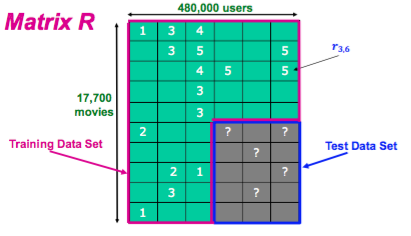
\includegraphics[width=1\linewidth]{figures/netflix_matrix.png}
  \caption{Netflix utility matrix}
  \label{fig:netflix_matrix}
\end{figure}

\paragraph{Bellkor solution.} Multi-scale modeling of the data
\begin{itemize}
  \item Global: mean rating overall users plus average difference of the user, to have a baseline
  \item Factorization: address regional effect
  \item Local neighborhood: related movies
  \item An idea is to embed the movies in a multi dimension vector space: Latent Factor Models (e.g. SVD)
\end{itemize}
